\documentclass{beamer}

% {{{ beamer stuffs
\setbeamertemplate{footline}[frame number]
\beamertemplatenavigationsymbolsempty%
\logo{
\includegraphics[height=4mm]{fig/LogoEnseeiht.png}}
\usetheme{Montpellier}
\usecolortheme{dolphin}
% }}}

\usepackage{fontspec}
\usepackage{hyperref}
\usepackage{pdflscape}

\usepackage{tikz}
\usetikzlibrary{shapes}

\title{CRAPS Kernel}
\subtitle{Final presentation}
\author{
       Maxime Arthaud
  \and Korantin Auguste
  \and Martin Carton
  \and Étienne Lebrun
}
\titlegraphic{
\includegraphics[width=0.5\textwidth]{fig/LogoEnseeiht.png}}
\date{March 13, 2015}

\begin{document}
  \begin{frame}[plain]
    \titlepage%
  \end{frame}

  \begin{frame}[plain]
    \tableofcontents
  \end{frame}

  \section{The project}
    \begin{frame}{Presentation}
      \begin{itemize}
        \item Implement a basic operating system on CRAPS:
          \begin{itemize}
            \item processor architecture developed by Jean-Christophe
              Buisson for first year students
            \item runs on a Nexys2 board
          \end{itemize}
        \item Goal: make a operating system course
          \begin{itemize}
            \item based on what student know
            \item adding a continuity in courses
            \item showing students how a basic operating system works
          \end{itemize}
      \end{itemize}
    \end{frame}

    \begin{frame}[label=big_picture]
      \begin{figure}
        \centering
        \includegraphics[height=\textheight]{build/big_picture_fromsvg.pdf}
      \end{figure}
    \end{frame}

    \begin{frame}[plain]
      \begin{figure}
        \centering
        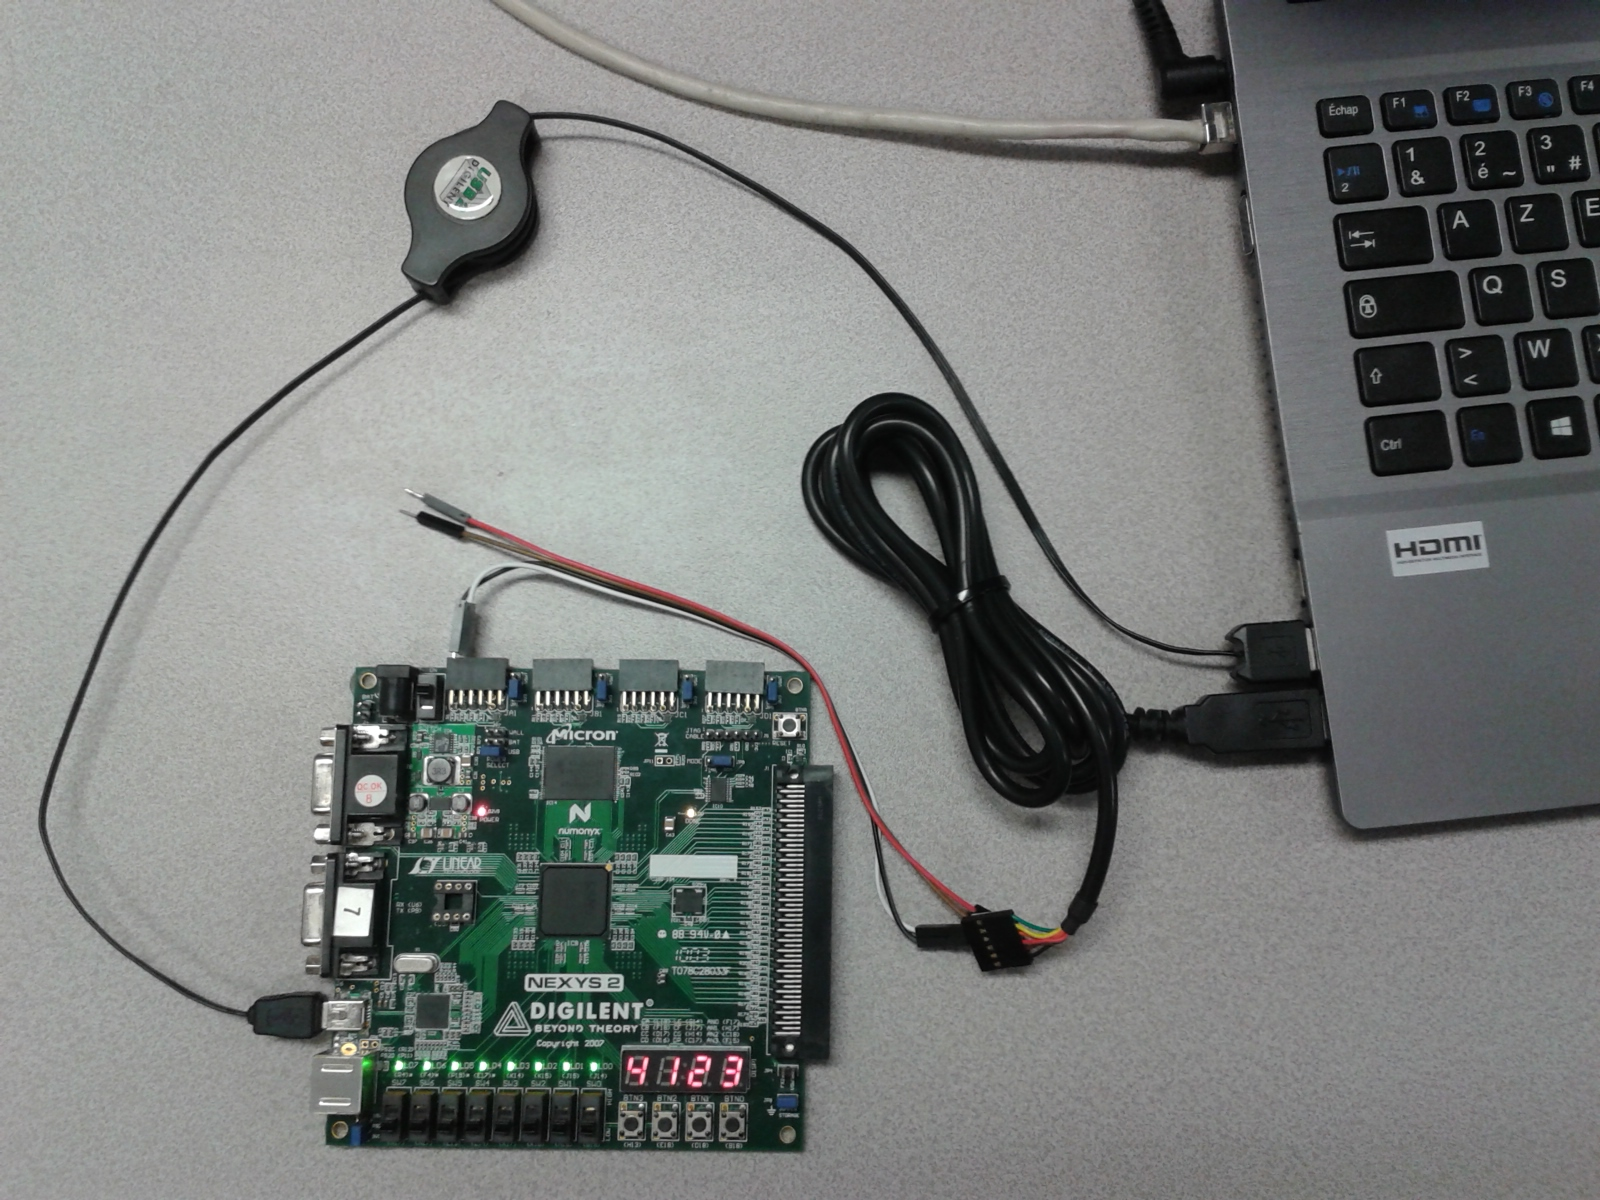
\includegraphics[width=\textwidth, keepaspectratio]{fig/Nexys2.jpg}
        \caption{A Nexys2 board}
      \end{figure}
    \end{frame}

  \section{Project Management}
    \subsection{Team}
      \begin{frame}{Team Organization}
        \begin{itemize}
          \item Korantin Auguste: responsible of development
          \item Maxime Arthaud: responsible of tests
          \item Martin Carton: project leader
          \item Étienne Lebrun: quality manager
        \end{itemize}
      \end{frame}

      \begin{frame}{Team Management}
        Quite free, working on what we like, when we like.

        \pause
        \begin{figure}
          \centering
          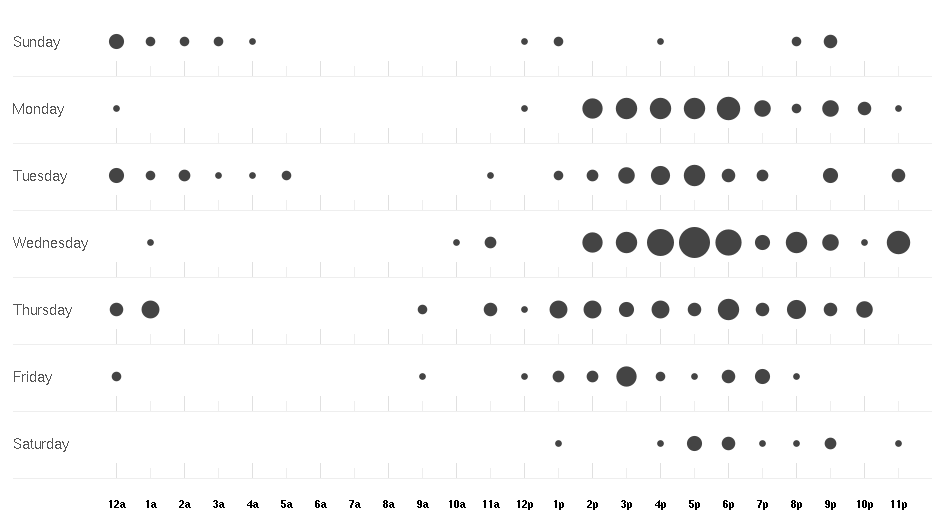
\includegraphics[width=0.9\textwidth]{fig/punchcard.png}
        \end{figure}
      \end{frame}

    \subsection{Project Organization}
      \begin{frame}{Risks Management}
        We have identified three risks and mitigated them:
        \begin{itemize}
          \item A FPGA might be damaged: we need more
          \item The OS might be too big to fit in the memory: we will need more
          \item The serial port might be too slow
        \end{itemize}
      \end{frame}

      \begin{frame}{Actions Management}
        We used a spreadsheet to manage the actions:
          \includegraphics[width=0.9\textwidth,keepaspectratio]
                          {Actions/ActionManagement.pdf}
      \end{frame}

      \begin{frame}{Specifications}
        \begin{itemize}
          \item First week of the project
          \item We identified three main tasks:
            \begin{itemize}
              \item The compiler
              \item The modifications to the processor
              \item The kernel
            \end{itemize}
          \end{itemize}
      \end{frame}

      \begin{frame}{Task Repartition and Planning}
          We used an incremental process, adding features one after another:%
          \begin{enumerate}
            \item Write a simple scheduler
            \item Add communications using serial port
            \item Handle dynamic program loading
          \end{enumerate}

          We wrote a planning taking finish-to-start constraints into account.
      \end{frame}

      \begin{frame}[plain]
        \begin{figure}
          \includegraphics[height=\textheight, width=\textwidth, keepaspectratio]
                          {build/Gantt.pdf}
        \end{figure}
      \end{frame}

      \begin{frame}{Test Means}
        Not fully automated because of the constraints of the project:
        \begin{itemize}
          \item hardware: need to manually load test code and test it via the
            monitor
          \item compiler: some automated tests test the compiler itself, but the
            generated code has to be tested manually and it is impossible to be
            exhaustive
          \item kernel: need to use the monitor as well, outputs use 7-segment
            display, switches, etc.
        \end{itemize}

        Creation of a command line tool to load code more easily.
      \end{frame}

      \begin{frame}{Deliverables}
        \begin{itemize}
          \item Documentation and manual for students and teachers
            \begin{itemize}
              \item What we changed
              \item How to use our tools
              \item The syntax of our language
              \item \dots
            \end{itemize}
          \item Kernel, compiler, new processor
          \item Reports, abstracts
          \item Software Development Plan, Specifications, Test Plan
        \end{itemize}
      \end{frame}

  \section{Implementation}
    \againframe{big_picture}

    \subsection{Kernel}
      \begin{frame}{Kernel introduction}
        Purpose of a kernel:
        \begin{itemize}
          \item Process management (scheduling)
          \item I/O (communication)
          \item Memory management (dynamic allocation)
        \end{itemize}
      \end{frame}

      \begin{frame}{Shell}
          We need to interact with the OS from the computer:
          \begin{itemize}
            \item Launch/stop programs
            \item Know the state of the processes
          \end{itemize}
      \end{frame}

      \begin{frame}{Scheduler}
        Needed for time sharing, to run multiple process in ``parallel'' on the
        CPU.

        \begin{figure}
            \centering
            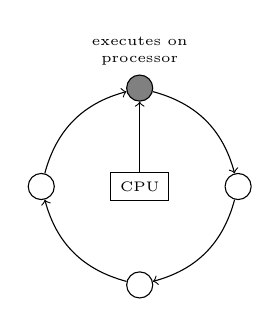
\begin{tikzpicture}[auto, ->, node distance=1.25cm]
            \node[auto] (CPU) [draw, style={font=\tiny}] {CPU};

            \node[auto] (A)   [draw, ellipse, above of=CPU, fill=gray,
            label={[align=center, style={font=\tiny}]executes on\\processor}] {};
            \node[auto] (B)   [draw, ellipse, right of=CPU] {};
            \node[auto] (C)   [draw, ellipse, below of=CPU] {};
            \node[auto] (D)   [draw, ellipse, left  of=CPU] {};

            \path (CPU) edge (A);

            \path (A) edge [bend left] (B);
            \path (B) edge [bend left] (C);
            \path (C) edge [bend left] (D);
            \path (D) edge [bend left] (A);
            \end{tikzpicture}
        \end{figure}

        Needed to make ``context switch'': change the current process. Via an interrupt called at a fixed frequency.
      \end{frame}

      \begin{frame}{Dynamic loading}
        We need to dynamically load a program:
        \begin{itemize}
          \item Dynamically allocate memory
          \item I/O communication to load the code
          \item Position independent code
        \end{itemize}
      \end{frame}

      \begin{frame}{Memory Management}
        \begin{itemize}
          \item We need to be able to dynamically allocate memory
          \item In modern computers: virtual memory (segmentation and pagination)
            \begin{itemize}
              \item Too complicated
            \end{itemize}
          \item We just need three functions: \texttt{malloc}, \texttt{free},
            \texttt{realloc}
        \end{itemize}
      \end{frame}

      \begin{frame}[plain]
        \begin{figure}
          \begin{minipage}[c]{0.5\textwidth}
            \caption{Memory layout}
          \end{minipage}\hfill
          \begin{minipage}[c]{0.5\textwidth}
            \includegraphics[height=\textheight]{build/memory_layout_fromsvg.pdf}
          \end{minipage}
        \end{figure}
      \end{frame}

    \subsection{Processor Changes}

          \begin{frame}{Extending the Processor}
          Pre-existing version of CRAPS not totally adapted to our needs:
          \begin{itemize}
            \item Not enough memory
            \item No external communications
            \item No proper interrupts
          \end{itemize}
      \end{frame}

      \begin{landscape}
        \begin{frame}[plain]
            \includegraphics[scale=0.22]
                            {build/micromachine_old_fromsvg.pdf}

        \end{frame}
        \begin{frame}[plain]
            \includegraphics[scale=0.22]
                            {build/micromachine_updated_fromsvg.pdf}

        \end{frame}
      \end{landscape}

      \begin{frame}{Original Sequencer}
          \begin{figure}
            \centering
            \makebox[\textwidth][c]{
              \includegraphics[scale=0.3]
                                {build/sequencer_old_fromsvg.pdf}
            }
          \end{figure}
      \end{frame}

      \begin{frame}{After updates}
        \begin{figure}
          \centering
          \makebox[\textwidth][c]{
            \includegraphics[scale=0.21]
                           {build/sequencer_updated_fromsvg.pdf}
          }
        \end{figure}
      \end{frame}

      \begin{frame}{Adding Memory}
          Three possibilities:
          \begin{itemize}
            \item Extend the RAM module inside the FPGA
                \begin{itemize}
                  \item 512 instructions $\implies$ more than 12.000
                \end{itemize}
            \pause
            \item Try to use the flash memory
            \pause
            \item Access the external 16Mb RAM chip
        \end{itemize}

      \end{frame}

      \begin{frame}{External Memory}
        \begin{itemize}
          \item Caution!
          \item Quite complex communication protocol
        \end{itemize}
        \pause
        Flash more complex than anticipated → Reorganisation of the planning
        
        Finally, does not suit our needs because of inherent limitations
        \pause

        We were able to integrate the external RAM, solving our memory issue
      \end{frame}

      \begin{frame}{Serial Port}
        To communicate with the computer we used a serial port.

        \pause
        We had to modify the processor:
        \begin{itemize}
          \item Add a new built-in module in SHDL
          \item Add a new interrupt in the processor
          \item Map the module to memory
        \end{itemize}

        \pause
        We had some problems:
        \begin{itemize}
          \item the module can cause the synthesis to fail (too complex?)
          \item the communication is slow, we can lose data
        \end{itemize}
      \end{frame}

      \begin{frame}{Interrupts}
        An interrupt is used to stop the execution of a task when some event
        happens:
        \begin{itemize}
          \item the PWM clock ticks → used to execute the scheduler at regular
            interval
          \item we receive a byte through the serial port → we need to save it
            before another comes
          \item etc.
        \end{itemize}

        \pause

        We had to add the interrupt system:
        \begin{itemize}
          \item Add an interrupts module, that keeps the state of each interrupt
          \item Use a priority encoder
        \end{itemize}
      \end{frame}

    \subsection{Compiler}
      \begin{frame}{Why we need a compiler}
        \begin{figure}
          \centering
          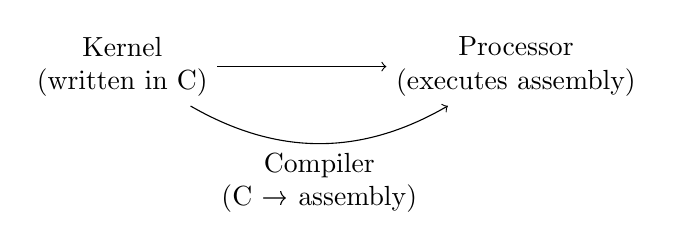
\begin{tikzpicture}[auto, ->, node distance=5cm]
            \node[auto] (K) [align=center] {Kernel\\(written in C)};
            \node[auto] (C) [right of=K, align=center]
                            {Processor\\(executes assembly)};

            \path (K) edge (C);
            \path (K) edge [bend right]
                      node [align=center, below] {Compiler\\(C → assembly)}
                  (C);
          \end{tikzpicture}
        \end{figure}

        \begin{itemize}
          \item We can't possibly write all the operating system in CRAPS
            assembly
          \item More practical for the student to code than assembly
        \end{itemize}

        The compiler is based on our second-year courses and the compiler
        generator of Mr.\ Gandriau: EGG.
      \end{frame}

      \begin{frame}{Modifications of The Second Year's Compiler}
        \begin{itemize}
          \item Generate CRAPS assembly
          \item A more complete language
          \item Various optimizations
          \item Position independent code for the dynamic loading
        \end{itemize}
      \end{frame}

  \section{Final Result}
    \subsection{Demonstration}
      \begin{frame}{Demo}
        \begin{itemize}
          \item The CRAPS processor is already on the board
          \pause
          \item Loading the kernel using the monitor
        \end{itemize}
        \begin{figure}
          \centering
          \makebox[\textwidth][c]{
            \includegraphics[width=10.5cm]{build/demo_load_fromsvg.pdf}
          }
        \end{figure}
        \pause
        \begin{itemize}
          \item Using the serial port with the shell task
          \pause
          \item Load a dynamic task
        \end{itemize}
      \end{frame}

  \section{Conclusion}
    \begin{frame}{Improvements}
      \begin{itemize}
        \item Integrate the flash chip to have persistent memory
        \item Use a better memory allocation strategy
      \end{itemize}
    \end{frame}

    \begin{frame}{Conclusion}
      \begin{itemize}
        \item The project was a success
        \item We really appreciated working on it
        \item We really hope future students will like it too
      \end{itemize}
    \end{frame}

  \section*{Questions}
    \begin{frame}
      Any questions?
    \end{frame}
\end{document}
